% Created 2025-05-28 Wed 14:19
\documentclass[compress,dvipdfmx,11pt]{beamer}
\usepackage[T1]{fontenc}
\usepackage{graphicx}
\usepackage{amsmath}
\usepackage[normalem]{ulem}
\usepackage{hyperref}
\title[2025年 大崎研究室ゼミ]{\bf はじめてのスライド作り}
\author[]{XXX XXX, 山近 駿}
\institute{関西学院大学 工学部 情報工学課程}
\date{2016 年 5 月 28 日}
\setlength{\parskip}{1.5ex}
\renewcommand{\textbf}{\alert}
\usetheme{Ohsaki}
\begin{document}

\maketitle
\begin{frame}{発表の内容}
\tableofcontents
\end{frame}

\newcommand{\pivec}{\mathbf \pi}
\newcommand{\xvec}{\mathbf x}
\newcommand{\yvec}{\mathbf y}
\newcommand{\zvec}{\mathbf z}
\newcommand{\Emat}{\mathbf E}
\newcommand{\Imat}{\mathbf I}

\bf

\section{はじめに}
\label{sec:org0f109a5}

\begin{frame}[label={sec:orge203cf1}]{研究の背景}
\begin{itemize}
\item あれが大事
\begin{itemize}
\item これも大事
\item そこでそれが必要
\end{itemize}
\item ところでこれは?
\begin{itemize}
\item あれも必要
\end{itemize}
\end{itemize}
\end{frame}

\begin{frame}[label={sec:org22aa2db}]{研究の目的}
\begin{enumerate}
\item あれをする
\item それをする
\item それもする
\end{enumerate}
\begin{align}
T = \frac{MSS \, \sqrt{1.5}}{R \, \sqrt{p}}
\end{align}
\end{frame}

\section{解析モデル}
\label{sec:orgd6eb59f}

\begin{frame}[label={sec:orga6a5bb4}]{解析モデル}
\begin{center}
\begin{center}
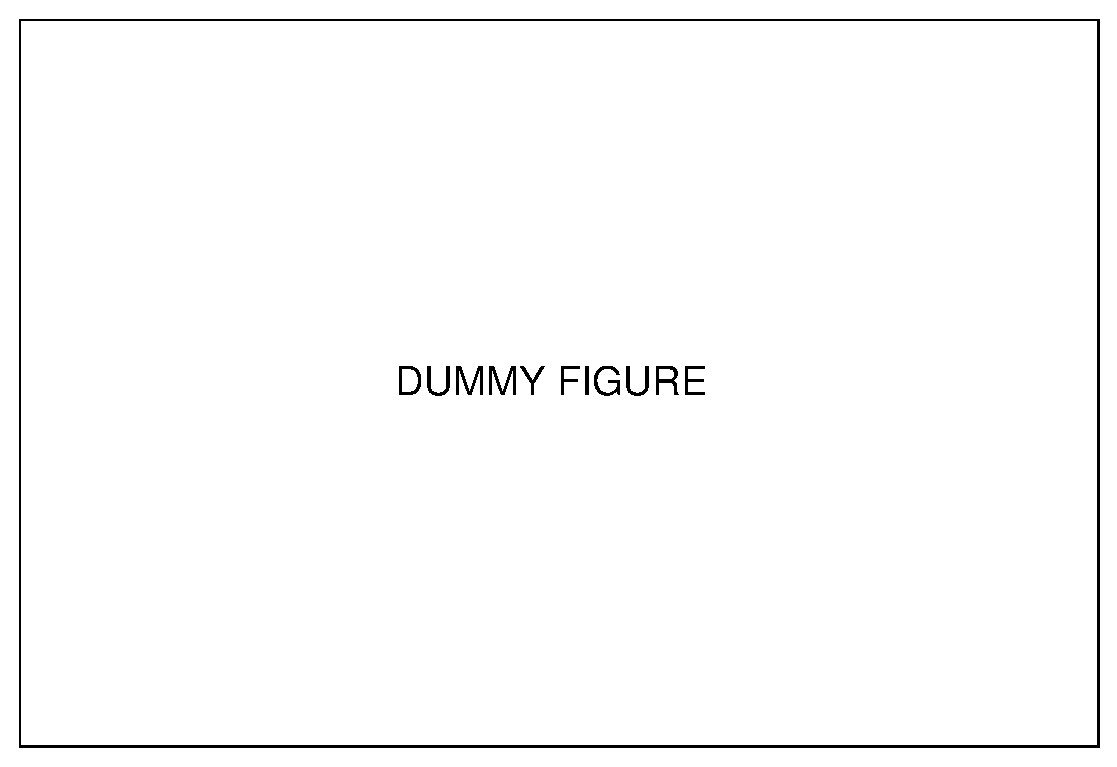
\includegraphics[width=\columnwidth]{./figure/dummy.eps}
\end{center}
\end{center}
\end{frame}

\begin{frame}[label={sec:orgf7be54e}]{解析における仮定}
\begin{columns}
\begin{column}{0.5\columnwidth}
\begin{itemize}
\item \(T\): スループット
\begin{itemize}
\item あれを含む
\end{itemize}
\item \(R\): ラウンドトリップ時間
\begin{itemize}
\item 時間がたっても変化しない
\end{itemize}
\end{itemize}
\end{column}

\begin{column}{0.5\columnwidth}
\begin{itemize}
\item \(T\): スループット
\begin{itemize}
\item あれを含む
\end{itemize}
\item \(R\): ラウンドトリップ時間
\begin{itemize}
\item 時間がたっても変化しない
\end{itemize}
\end{itemize}
\end{column}
\end{columns}
\end{frame}

\section{解析}
\label{sec:orgc9555a4}

\begin{frame}[label={sec:org5b80ffa}]{キャッシュヒット率の導出}
\begin{align}
T = \frac{MSS \, \sqrt{1.5}}{R \, \sqrt{p}}
\end{align}
\end{frame}

\begin{frame}[label={sec:org2608ff3}]{メッセージ配送遅延の導出}
\begin{align}
T = \frac{MSS \, \sqrt{1.5}}{R \, \sqrt{p}}
\end{align}
\end{frame}

\section{数値例}
\label{sec:org25bc202}

\begin{frame}[label={sec:orgc2b13c9}]{数値例: バッファサイズとスループットの関係}
\begin{center}
\begin{center}
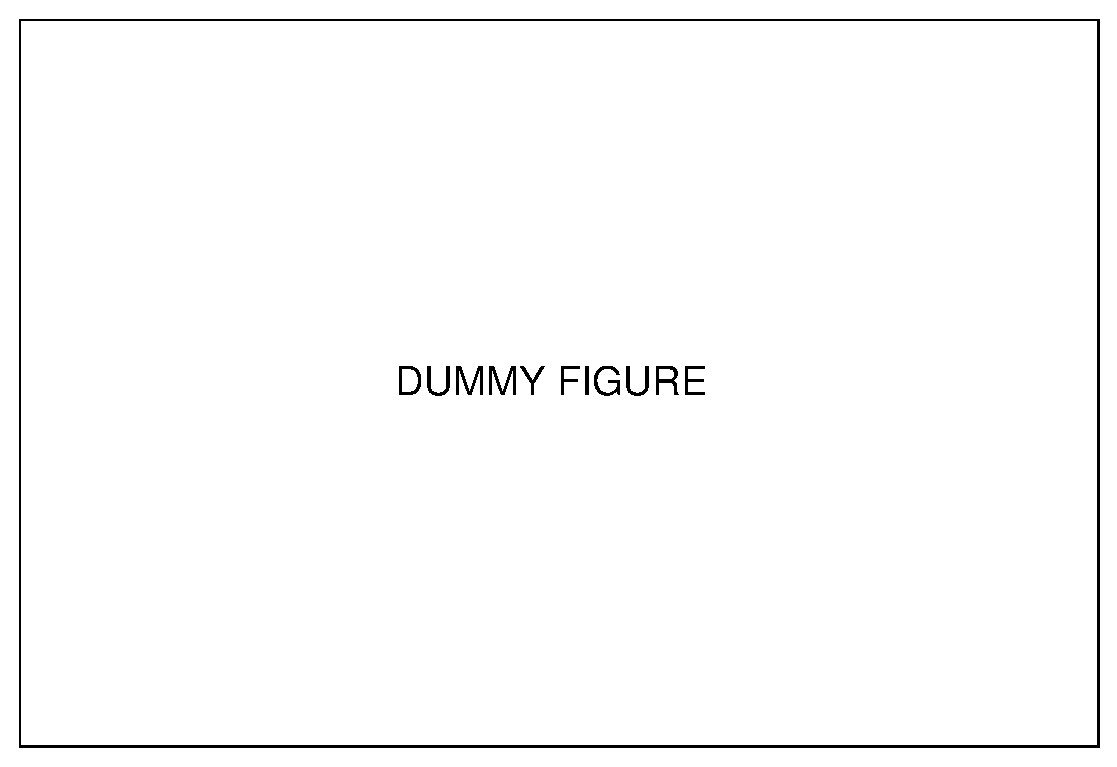
\includegraphics[width=.7\columnwidth]{./figure/dummy.eps}
\end{center}
\end{center}

\begin{center}
\(T\) = 12 [Mbit/s], \(B\) = 1,000 [byte], \(L\) = 1 [packet]
\end{center}
\end{frame}

\begin{frame}[label={sec:orgb2b22f7}]{数値例: バッファサイズとスループットの関係}
\begin{columns}
\begin{column}{0.5\columnwidth}
\begin{center}
\begin{center}
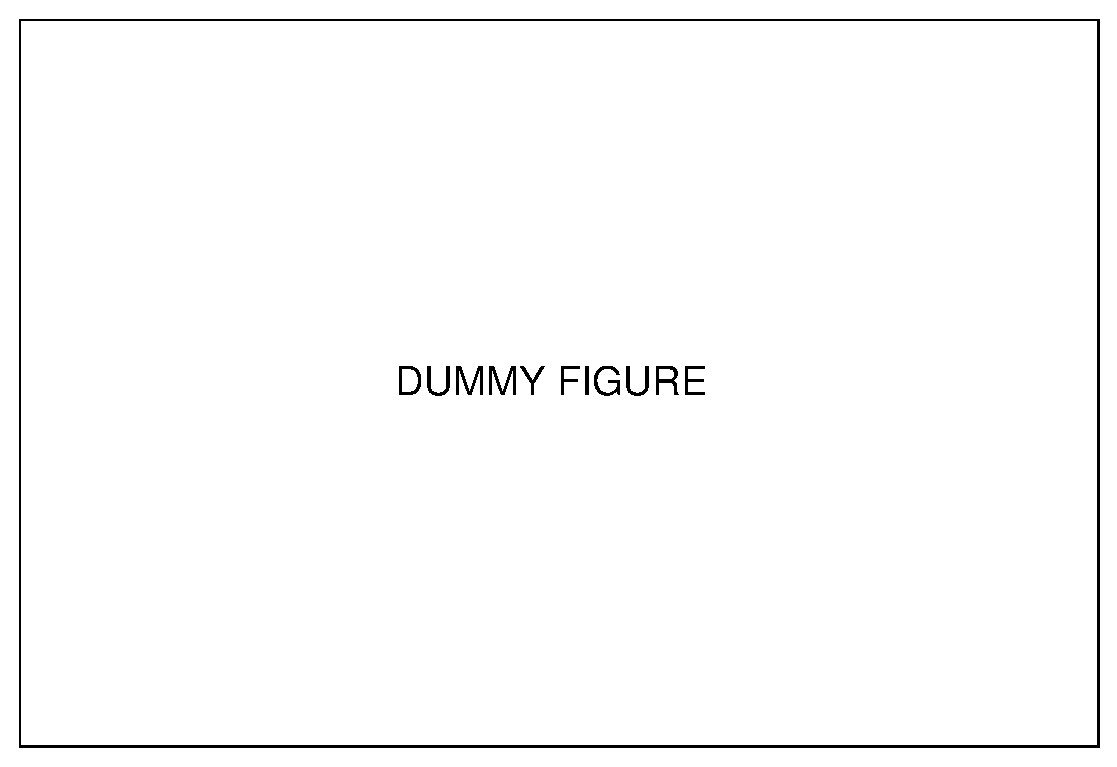
\includegraphics[width=\columnwidth,height=.7\textheight]{./figure/dummy.eps}
\end{center}
\end{center}
\end{column}

\begin{column}{0.5\columnwidth}
\begin{center}
\begin{center}
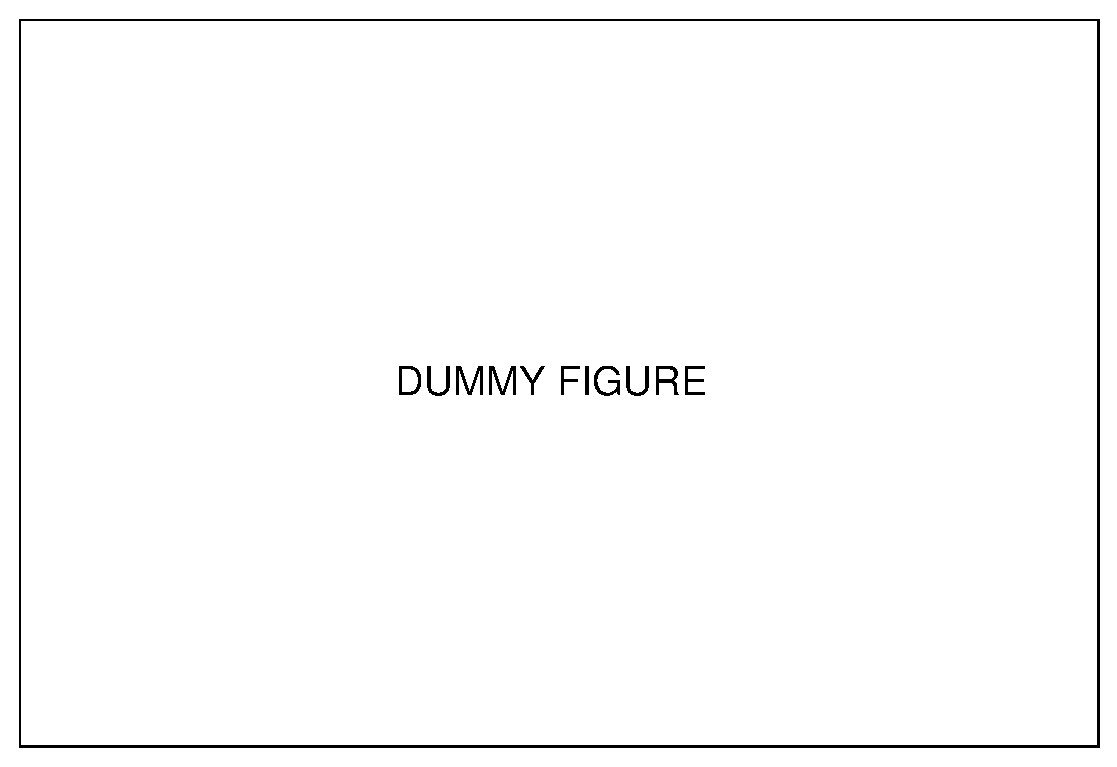
\includegraphics[width=\columnwidth,height=.7\textheight]{./figure/dummy.eps}
\end{center}
\end{center}
\end{column}
\end{columns}
\end{frame}

\section{まとめ}
\label{sec:orgc84405a}

\begin{frame}[label={sec:org0755e16}]{まとめ}
\begin{itemize}
\item あれをした
\item これをした
\end{itemize}
\end{frame}

\begin{frame}[label={sec:org0012268}]{今後の課題}
\begin{itemize}
\item あれをしたい
\item これをしたい
\end{itemize}
\end{frame}
\end{document}